\documentclass[../main.tex]{subfiles}
\begin{document}
\section{Database}
A database is defined as a collection of data and the organization given to this data. The data is organized in tables, in which the data has no formatting. The main difference between a database and a simple spreadsheet is not only the lack of formatting in the database tables, but most importantly the presence of relation that define a structure between the database tables.\\
Data is related using common key (common fields) or common concepts. The use of a structure allow the database tables to be light, in the sense that each table can rely on another one and therefor avoid storing duplicated data allowing for scalability but also for a easiness in the way data is retrieved. 

\begin{figure}[H]
    \centering
\begin{tikzpicture}[scale=0.5, table/.style={matrix of nodes, nodes in empty cells, column sep=-\pgflinewidth, row sep=-\pgflinewidth, nodes={draw,anchor=center,minimum width=2.5cm,minimum height=1cm}, row 1/.style={nodes={minimum height=1cm}}}]
\matrix(User) [table, label=above:Users] {
    \textbf{ID} & \textbf{Name} & \textbf{Surname} \\ 1 & Mario & Rossi \\ 2 & Frank & Weber \\};
\matrix(Time worked) [table, label=above:Time table, right=1cm of User] {
    \textbf{ID} & \textbf{Time [h]} \\ 1 & 4 \\ 2 & 6 \\ 1 & 3 \\ 2 & 8 \\ 2 & 9 \\};
\draw (User-3-1.south)--++(0,-3.5)-|(Time worked-6-1);
\end{tikzpicture}
    \caption{Database Example}
    \label{fig:dbexample}
\end{figure}
\begin{figure}[H]
\begin{center}
\begin{tabular}{ | m{2.5cm} | m{2.5cm}| m{2.5cm} | } 
\hline
\textbf{Name} & \textbf{Surname} & \textbf{Time [h]} \\ 
\hline
Mario & Rossi & 4 \\
\hline
Frank & Weber & 6 \\
\hline
Mario & Rossi & 3 \\
\hline
Frank & Weber & 8 \\
\hline
Frank & Weber & 9 \\
\hline
\end{tabular}
\end{center}
    \caption{Spreadsheet like organization}
    \label{fig:spreadsheet}
\end{figure}
In order to better visualize the actual effectiveness of a database an example is presented. The same data is reported in a database like way in Fig. \ref{fig:dbexample} and in a spreadsheet like manner in Fig. \ref{fig:spreadsheet}. At first sight, the spreadsheet seems to have less data, indeed no ID is presents making the visualization cleaner. The example is basic and the lack of high volume data makes it hard for the database structure to effectively pop out. Consider now that all the cell require the same storage capacity in terms of memory (i.e. string and integers require the same space in memory), the function governing the number of total cells is for the example in \ref{fig:spreadsheet}:
\begin{equation}
    tot = time_{entries} \cdot 3
\end{equation}
While for the case reported in \ref{fig:dbexample}:
\begin{equation}
    tot = time_{entries} \cdot 2 + ID_{unique} \cdot 3
\end{equation}
\begin{figure}[H]
    \centering
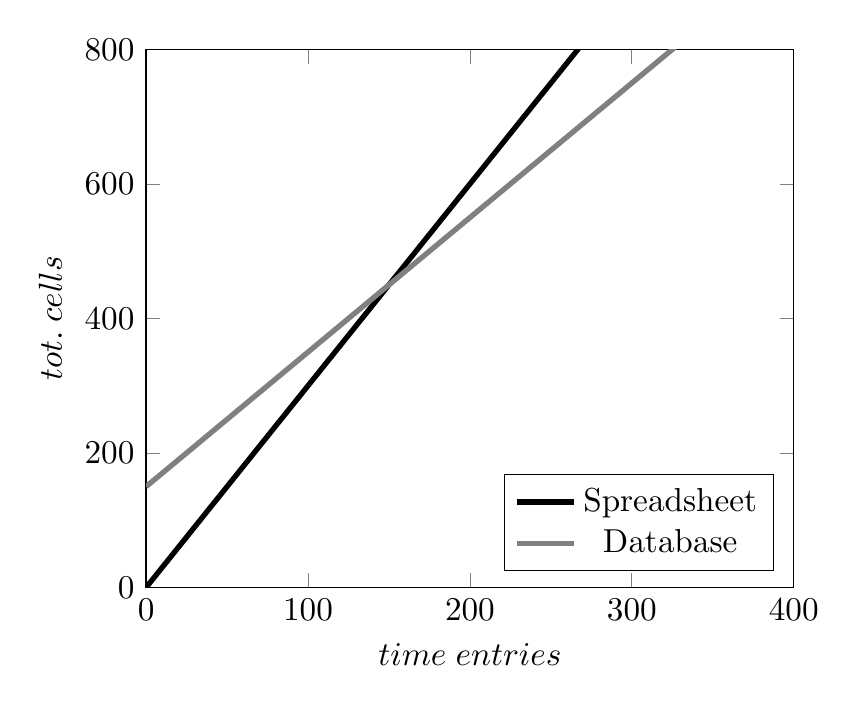
\begin{tikzpicture}[scale=1.2]
\begin{axis}[xmin=0, ymin=0, xmax=400, ymax=800, samples= 100, xlabel=$time\;entries$,ylabel=$tot.\;cells$, legend pos=south east]
  \addplot[black, ultra thick, domain=0:1000] (x,3*x);
  \addplot[gray,  ultra thick, domain=0:1000] (x,2*x + 3*50);
  \addlegendentry{Spreadsheet}
  \addlegendentry{Database}
\end{axis}
\end{tikzpicture}
    \caption{Comparison with 50 User}
    \label{fig:my_label}
\end{figure}
It´s easy from the plot, that consider a fixed number of 50 Users that the structure solution comes to be the most effective one as the data increase. This is also most efficient when a single entry is comprised by more instances, not only 2 as in this case (Name, Surname). A structured database bring others benefits to the picture, such as:
\begin{itemize}
    \item Data accessibility and speed, database integrate querying functionality that can retrieve data based on certain criteria, perform aggregate and calculation across multiple different tables. Other than that the access mechanism is faster than the spreadsheet one, related to the way database data is saved in the memory. 
    \item Data Integrity, in database strict rules are defined for the tables in order to ensure that at the data is accurate and accessible. Relationship between data (ID in \ref{fig:dbexample}) and other matching mechanism as primary keys are part of what´s defined \textit{referential integrity}.
    \item Redundancy avoidance, in database, as can be grasped for the example the structure allow for a reduction of redundancy. Duplicates data mean there is a lacking structure. 
    \item Accessibility, database are meant to be worked on by multiple people in a concurrent manner, differently from spreadsheets. This mean a structured user hierarchy is determined in the database. 
\end{itemize}

\subsubsection{Types of databases}
\subsection{Creation of a connection to database on a server}
\subsection{SQL Database}
\subsubsection{Primary key and foreign key}
\section{Slq alchemy}
\subsubsection{ORM Layer}
\subsection{Tables object}
\section{Database update mechanism}
\cleardoublepage
\end{document}